\documentclass{beamer}
\usepackage[latin1]{inputenc}
%\usetheme{Montpellier}
\usetheme{Boadilla}
\usepackage{color, colortbl}
%\usecolortheme[RGB={204,51,255}]{structure}
%\usecolortheme[named=plum]{structure}
\usecolortheme[RGB={62,128,62}]{structure}
%\definecolor{dark}{rgb}{0.3,0.15,0.3}
%\definecolor{light}{rgb}{0.8,0.6,0.8}
\definecolor{reddish}{rgb}{0.15,0.5,0.15}
\definecolor{dark}{rgb}{0.4,0.2,0.4}
\definecolor{darkgreen}{rgb}{0.25,0.5,0.25}
\definecolor{darkred}{rgb}{0.75,0.25,0.25}
\definecolor{darkblue}{rgb}{0.25,0.25,0.75}
\definecolor{light}{rgb}{0.8,0.6,0.8}
\definecolor{darklight}{rgb}{0.6,0.45,0.6}
\definecolor{newlight}{rgb}{0.6,0.8,0.8}
\definecolor{newdarklight}{rgb}{0.45,0.6,0.6}
\definecolor{reddish}{rgb}{.7,0.25,0.25}
\usepackage{graphicx}
\usepackage{pstricks}

\usepackage{listings}
%%
%% Julia definition (c) 2014 Jubobs
%%
\lstdefinelanguage{Julia}%
  {morekeywords={abstract,break,case,catch,const,continue,do,else,elseif,%
      end,export,false,for,function,immutable,import,importall,if,in,%
      macro,module,otherwise,quote,return,switch,true,try,type,typealias,%
      using,while},%
   sensitive=true,%
   alsoother={$},%
   morecomment=[l]\#,%
   morecomment=[n]{\#=}{=\#},%
   morestring=[s]{"}{"},%
   morestring=[m]{'}{'},%
}[keywords,comments,strings]%

\lstset{%
    language         = Julia,
    basicstyle       = \ttfamily,
    keywordstyle     = \bfseries\color{blue},
    stringstyle      = \color{magenta},
    commentstyle     = \color{ForestGreen},
    showstringspaces = false,
}


\setbeamertemplate{navigation symbols}{}


\newcommand{\cored}{\color{red}{}}
\newcommand{\coblu}{\color{blue}{}}
\newcommand{\coblue}{\color{blue}{}}
\newcommand{\cor}{\color{reddish}{}}
\newcommand{\cob}{\color{black}{}}

\newcommand*\eiadfamily{\fontencoding{OT1}\fontfamily{eiad}\selectfont}
\usepackage[OT1]{fontenc}




\title[Chapter 1]{Chapter 1 - Examples}
\author{Conor Houghton}
\institute{reading Gelman}
\date{(2022-01-27) bayesianreadinggroup.github.io}

\begin{document}

\maketitle

\begin{frame}[fragile]{Football data}
\texttt{http://www.stat.columbia.edu/$\sim$gelman/book/data/}

\begin{verbatim}
home favorite underdog spread name1 name2 week
 1  21  13    2.0  TB  MIN   1
 1  27   0    9.5  ATL NO    1
 1  31   0    4.0  BUF NYJ   1
 1   9  16    4.0  CHI GB    1
 1  27  21    4.5  CIN SEA   1
 0  26  10    2.0  DAL WAS   1
 1  24  17    5.0  DET SF    1
 1  20  27    6.0  LAN HOU   1
 0  20   7    1.0  MIA PHX   1
\end{verbatim}
\vfill
\color{gray}
(where name1 and name2 have been changed to fit)
\color{black}
\end{frame}


\begin{frame}[fragile]{Football data - some sed-foo}
\begin{verbatim}
sed 's/\s\+/,/g' football_data.txt
 | sed 's/,//'> football_data.csv
\end{verbatim}
\color{red}giving:\color{black}
\begin{verbatim}
home,favorite,underdog,spread,name1,name2,week
1,21,13,2.0,TB,MIN,1
1,27,0,9.5,ATL,NO,1
1,31,0,4.0,BUF,NYJ,1
1,9,16,4.0,CHI,GB,1
1,27,21,4.5,CIN,SEA,1
0,26,10,2.0,DAL,WAS,1
1,24,17,5.0,DET,SF,1
1,20,27,6.0,LAN,HOU,1
0,20,7,1.0,MIA,PHX,1
\end{verbatim}
\end{frame}

\begin{frame}[fragile]{Load DataFrame}
\begin{lstlisting}
using CSV, DataFrames

fD = DataFrame(CSV.File("football_data.csv"))

fD.diff  = fD.favorite - fD.underdog
fD.error = fD.spread   - fD.diff
\end{lstlisting}
\vfill
\color{gray}
(variable names shortened to fit; long names ftw)
\color{black}

\end{frame}

\begin{frame}[fragile]{Make the scatter plot}
    \lstset{emph={x,y},emphstyle=\color{red}}
  \begin{lstlisting}

using Gadfly,Cairo,Fontconfig

plt=plot(fD,x=:spread,y=:difference,
         Theme(default_color="red",
               point_size=1pt,
               background_color="white",
               highlight_width=0pt),
         Stat.x_jitter(range=0.5),
         Stat.y_jitter(range=0.5),
         Geom.point,
         Coord.Cartesian(xmin=-0.5,xmax=20.5)
         )
  \end{lstlisting}
  \end{frame}

\begin{frame}{Make the scatter plot}
  \begin{center}
  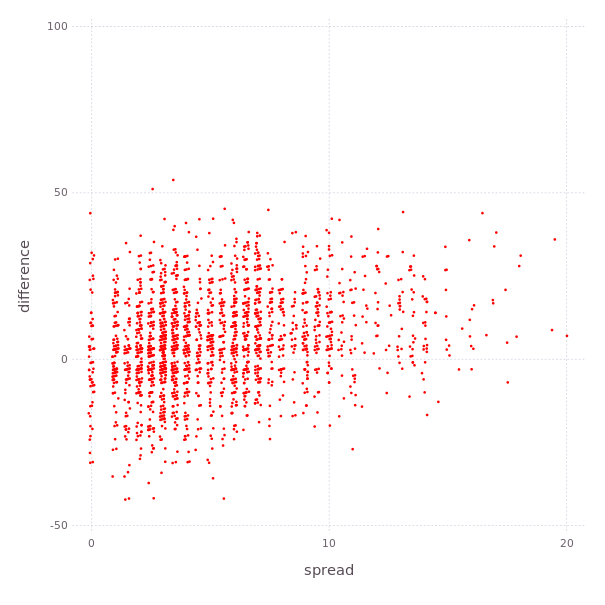
\includegraphics[width=8cm]{spreadVdiff.png}
\end{center}
  \end{frame}


\begin{frame}[fragile]{Are integer and half-integer spreads the same}
    \lstset{emph={x,y},emphstyle=\color{red}}
  \begin{lstlisting}
fD.integerSpread=round.(fD.spread).==fD.spread

mD = groupby(fD, :integerSpread)
mD = combine(mD, nrow, :error => mean => :mean)

\end{lstlisting}
\end{frame}


\begin{frame}[fragile]{Are integer and half-integer spreads the same}
    \lstset{emph={round},emphstyle=\color{red}}
  \begin{lstlisting}
fD.integerSpread=round.(fD.spread).==fD.spread

mD = groupby(fD, :integerSpread)
mD = combine(mD, nrow, :error => mean => :mean)

\end{lstlisting}
\end{frame}


\begin{frame}[fragile]{Are integer and half-integer spreads the same}
    \lstset{emph={integerSpread,error,mean},emphstyle=\color{red}}
  \begin{lstlisting}
fD.intSpread=round.(fD.spread).==fD.spread

mD = groupby(fD, :intSpread)
mD = combine(mD, nrow, :error => mean => :mean)

\end{lstlisting}
\end{frame}



\begin{frame}[fragile]{Are integer and half-integer spreads the same}
    \lstset{emph={integerSpread,error,mean},emphstyle=\color{red}}
  \begin{lstlisting}
layer1=layer(fD,x=:intSpread,y=:error,Geom.violin)
layer2=[stuff with mD to get mean bars]

plt=plot(layer2,layer1,
        Theme(background_color="white")
        )
\end{lstlisting}
\end{frame}


\begin{frame}{Are integer and half-integer spreads the same}
  \begin{center}
  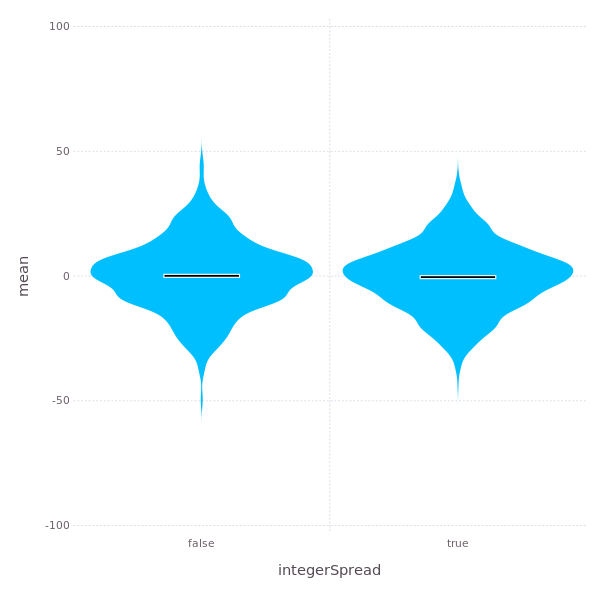
\includegraphics[width=8cm]{integerSpread.png}
\end{center}
  \end{frame}

\begin{frame}{Model}
\color{reddish}
  $$\mbox{difference} = \mbox{spread} + \xi$$
\color{black}where\color{reddish}
$$\xi\sim\mbox{Normal}(0,\sigma^2)$$
\color{black}and\color{reddish}{} $\sigma=14$\color{black}. This implies that a win happens with probability\color{reddish}
$$\mbox{Pr}(\mbox{difference}>0)=\mbox{Pr}(\xi<\mbox{score})$$
\color{black}which can be easily found by integrating the Gaussian and gives an error function up to the usual messing with the root of two.
\end{frame}


\begin{frame}[fragile]{Check predictions}
    \lstset{emph={integerSpread,error,mean},emphstyle=\color{red}}
  \begin{lstlisting}

model(spread,s) = 0.5+0.5erf(spread /(sqrt(2)*s))

w(a,b)= if(a>b) 1.0 elseif(a<b) 0.0 else 0.5 end
    
\end{lstlisting}
\end{frame}


\begin{frame}[fragile]{Check predictions}
    \lstset{emph={groupby,combine},emphstyle=\color{red}}
  \begin{lstlisting}

fD.win = w.(fD.favorite,fD.underdog)

wins = groupby(fD, :spread)
wins = combine(wins,nrow,:win => sum => :totalWin)

s=14.0

wins.counted = wins.totalWin ./ wins.nrow
wins.predicted = modelResult.(wins.spread,s)
    
\end{lstlisting}
\end{frame}


\begin{frame}{Check predictions}
  \begin{center}
    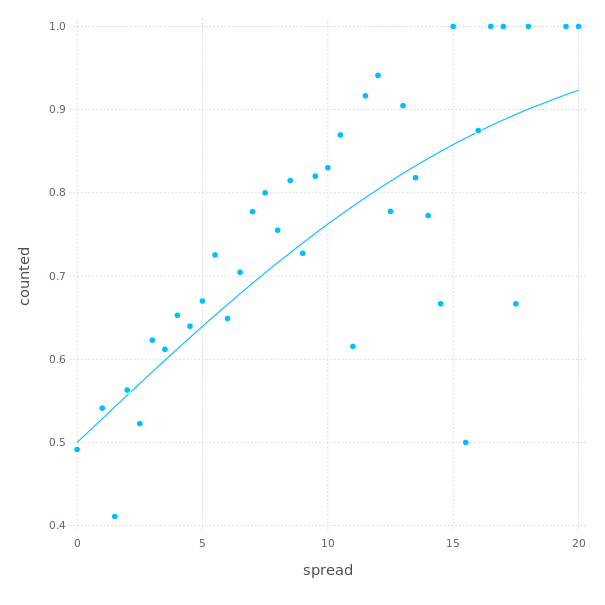
\includegraphics[width=8cm]{prediction.png}
\end{center}
  \end{frame}


\begin{frame}[fragile]{Check predictions}
    \lstset{emph={groupby,combine},emphstyle=\color{red}}
  \begin{lstlisting}

fD.win = score.(fD.favorite,fD.underdog)

wins = groupby(fD, :spread)
wins = combine(wins,nrow,:win => sum => :totalWin)

s=std(fD.error)

wins.counted = wins.totalWin ./ wins.nrow
wins.predicted = modelResult.(wins.spread,s)
    
\end{lstlisting}
\end{frame}


\begin{frame}{Check predictions}
  \begin{center}
    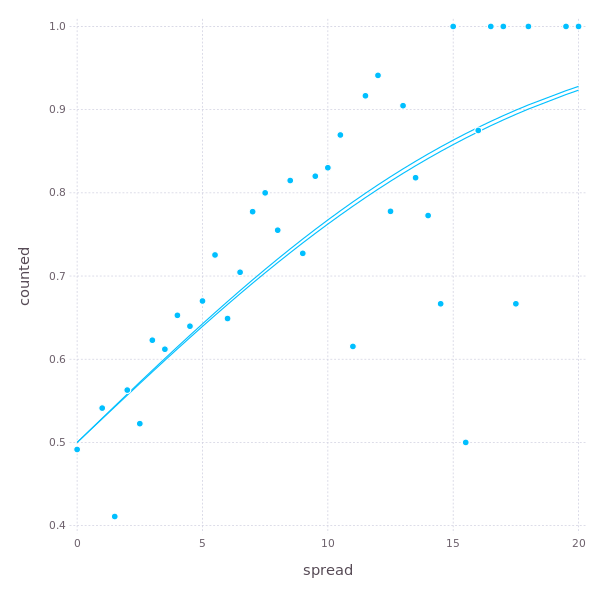
\includegraphics[width=8cm]{predictionNewSigma.png}
\end{center}
  \end{frame}


\begin{frame}{Check predictions - sigma}
  \begin{center}
    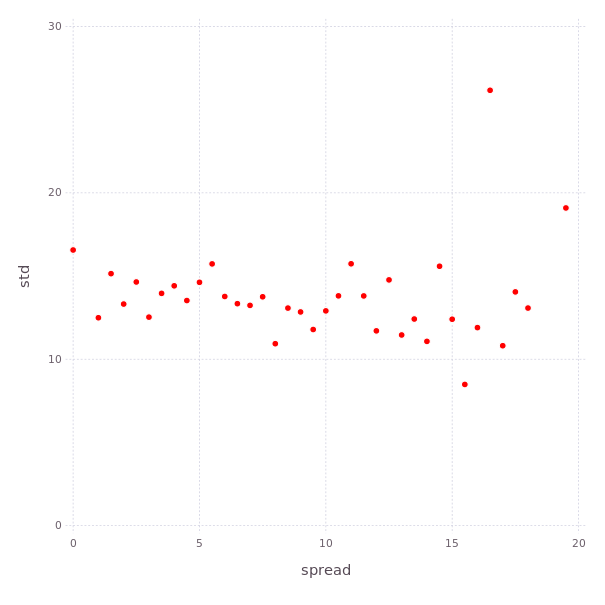
\includegraphics[width=8cm]{sigma.png}
\end{center}
  \end{frame}


\begin{frame}{Check predictions - color for data size}
  \begin{center}
    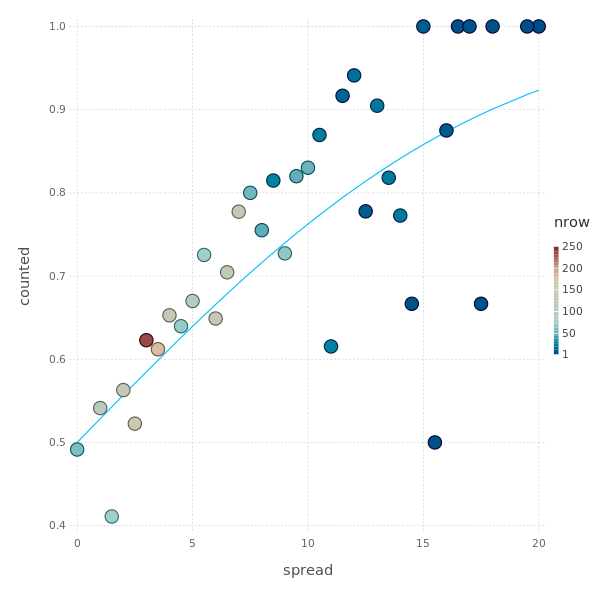
\includegraphics[width=8cm]{predictionColor.png}
\end{center}
  \end{frame}

\begin{frame}[fragile]{Filter for data size}
    \lstset{emph={findall,filter},emphstyle=\color{red}}
  \begin{lstlisting}

cutOff=100
cut=wins.spread[findall(x -> x>cutOff,wins.nrow)]
isGood(x) = x in cut

model = std(filter(:spread => isGood,fD).error)
    
\end{lstlisting}
\end{frame}


\begin{frame}{Check predictions - new sigma}
  \begin{center}
    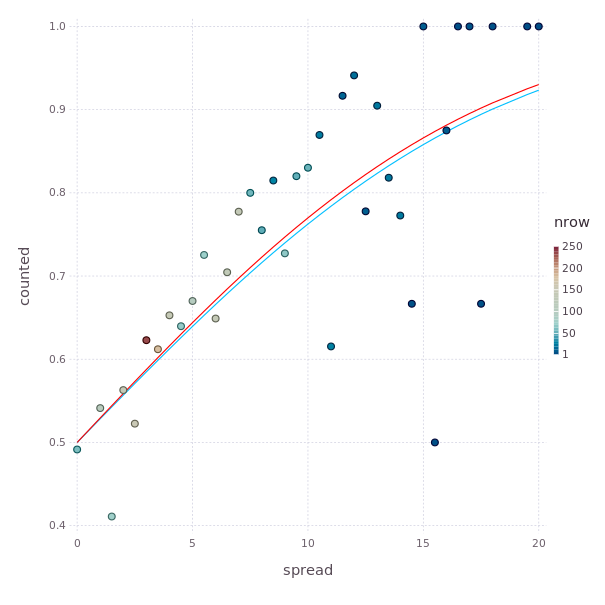
\includegraphics[width=8cm]{predictionGood.png}
\end{center}
  \end{frame}

\begin{frame}[fragile]{Regression}
      \lstset{emph={findall,filter},emphstyle=\color{red}}
  \begin{lstlisting}
using GLM
    
fm = @formula(difference ~ spread)
linearRegressor = lm(fm, fD)
    
\end{lstlisting}
\end{frame}

\begin{frame}[fragile]{Regression}
  \begin{verbatim}
difference ~ 1 + spread

Coefficients:
-----------------------
                Coef.  
-----------------------
(Intercept)  0.152845  
spread       1.0139    
-----------------------
\end{verbatim}
 \end{frame}

\begin{frame}{Another question}

\textbf{8}. \textbf{Subjective probability}: discuss the following
statement. `The probability of event $E$ is considered ``subjective''
if two rational persons $A$ and $B$ can assign unequal probabilities
to $E$, $P_A(E)$ and $P_B(E)$. These probabilities can also be
interpreted as ``conditional'':
$$P_A(E) = P(E|I_A)$$
and
$$P_B(E) = P (E|I_B)$$
where $I_A$ and $I_B$ represent the knowledge available to persons $A$ and $B$,
respectively.' Apply this idea to the following examples.
\begin{itemize}
\item[a] The probability that a `6' appears when a fair die is rolled, where $A$
  observes the outcome of the die roll and $B$ does not.
\item[b] The probability that Brazil wins the next World Cup, where $A$ is ignorant of soccer and $B$ is a knowledgeable sports fan.
  \end{itemize}
\end{frame}

\end{document}
